\section{Near Neighbor Search}\label{sec:nn}

Fast retrieval of similar patches is crucial for making
construction of a sizable patch-based database feasible.
This is essentially near-neighbor retrieval in
relatively high dimensions $3 \cdot n^2$ (1875 for patch size $n=25$).
Image retrieval has been addressed in a number of papers,
including more complex feature representations ~\cite{perronnin2010large}.
Our problem is somewhat different from most of previous work
in that the variability
in small patches is much less than in regular-sized images,
semantic information is irrelevant, and vectors are much shorter
than for regular-sized images.
Thus, we focus on tuning a simple Locality-Sensitive Hashing variant for our
particular application.

\subsection{Locality-Sensitive Hashing}

\begin{figure}[ht!]
\centering
\subfigure[Typical LSH uses several tables.]{
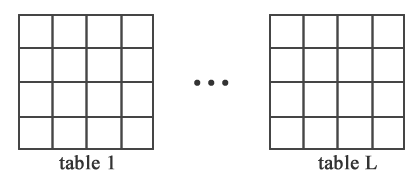
\includegraphics[width=3.0in]{fig_NN/lsh_tables.png}}
\subfigure[Random projection hashing family $\mathcal{F}$.]{
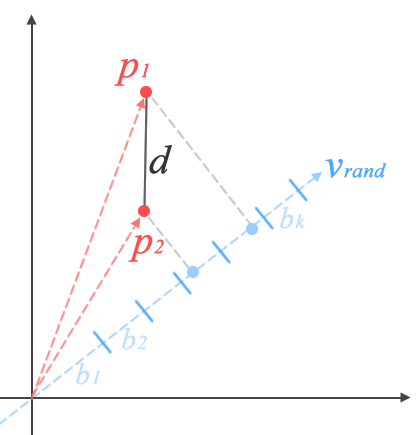
\includegraphics[width=2.5in]{fig_NN/rand_proj.png}}
\caption{a) LSH typically constructs
$L$ hash tables, each relying on an amplified
hash function $\mathcal{G}$, composed of a concatenation
of simpler hash functions $\mathcal{F}$. b) In
random projection hashing, each
$\mathcal{F}$ is evaluated by projecting a point $p$
(a patch color vector in our case) on a randomly chosen
unit vector, and binning it into uniform bins.}
\label{fig:lsh}
\end{figure}

Locality-Sensitive Hashing (LSH)~\cite{LSH:Andoni}
is a popular approach for approximate near-neighbor search
in high dimensions. The high-level idea behind LSH is
using a set of hashing functions that map
a vector $P_i$ to its bin $b(P_i)$ such that:
\begin{equation*}
\begin{aligned}
P[b(P_i) = b(P_j) | S(P_i, P_j) < T] > P_1\\
P[b(P_i) = b(P_j) | S(P_i, P_j) > cT] < P_2
\end{aligned}
\end{equation*}
where the collision probability
for vectors that are close together is high
($> P_1$), and the probability of collision
for vectors that are further apart is low ($< P_2$).

To achieve high guarantees on finding the nearest
neighbor, LSH typically requires multiple hash tables.
For example, two red points in Fig.~\ref{fig:lsh} are close,
but they fall in different bins in table 1. However,
in some table (say Table $L$), they are likely to end up in
the same bin. This amounts to taking an OR over
collisions in all the tables, amplifying probabilities.
Implementing this scenario in the context
of a database incurs a significant storage overhead, as for each
patch $P_i$ we not only need to store the patch itself,
but also $L$ hash indices. By the same token,
queries must be made to all the hash tables, which incurs significant
overhead at near neighbor search time.

High precision near neighbor search is not necessary
for our application, and we focus, instead, on \emph{efficiency}.
In order to accomplish that we aim to \textbf{minimize the
probability of collision for dis-similar patches}, as long
as probability of collision for similar patches results in
finding enough neighbors for a suitable compression ratio.
To this end, we aim to answer the question:
\emph{how well can the system perform with just one hash table?}

In order to optimize the performance of our single hash table,
we want to \emph{amplify} the probability of a single hash
function from a family $\mathcal{F}$ by using an AND operator
on collisions with several hash functions
$\mathcal{F}_1...\mathcal{F}_q$ from that family.
This is a standard technique which results in an amplified
hash function $\mathcal{G}$:
\begin{equation}
\mathcal{G}(P_i) = \mathtt{ConcatBits}(\mathcal{F}_1(P_i),...,\mathcal{F}_q(P_i))
\end{equation}\label{eq:ampl}
\noindent where $\mathtt{ConcatBits}$ simply allocates a constant
number of bits to each hash and concatenates them into a single value.
The probability that dis-similar patches collide with
this amplified function is $(P_2)^q$, where $P_2$ is the
probability of collision using just one function in the family.
We formalize our Near Neighbor search in Sec.~\ref{ssec:nn-lsh},
and take a closer look at hashing functions in the following sections.
In Sec.~\ref{ssec:naive-nn}, we introduce a common choice for a
 hash function family $\mathcal{F}$, and optimize it for our application in Sec.~\ref{ssec:pca-nn}
and \ref{ssec:uni-nn}.

\subsection{Near-Neighbor Search with LSH}\label{ssec:nn-lsh}

Using a single amplified hash function $\mathcal{G}$, finding
all likely neighbors of a patch simply amounts to computing
its hash value and taking all the patches that fall into the
same hash bin.
More formally, we define our approach
in alg.~\ref{alg:insert2} as follows:
\begin{algorithmic}[1]
\Statex \texttt{\textbf{FindLikelySimilarPatches}}($P_j$):
\State $h \leftarrow \mathcal{G}$ (\texttt{ToVector($P_j$)})
\State $SimPat \leftarrow$ \texttt{select patch from patch\_dict where id in
(select patch\_id from patch\_hashes where hash = h)}
\end{algorithmic}
Of course, the quality of the result depends heavily on the
properties of the hash function, which is something we discuss next.

\subsection{Random Projections Hashing}\label{ssec:naive-nn}

A common choice for a hash function family $\mathcal{F}$ is
the family of random projection functions. In this scheme,
a given $\mathcal{F}_i(P_j) \in \mathcal{F}$ is evaluated by
projecting $P_j$ onto a randomly chosen unit vector $v_i$,
and binning the value into a randomly chosen bin (see fig.~\ref{fig:lsh},
where bins are uniform across dot product values:
\begin{equation}
\mathcal{F}_i(P_j) = \floor{\frac{P_i \cdot \mathbf{v}_i + b}{w}}
\end{equation}
We choose to work with this approach, but operate under
the constraint that the value of the amplified $\mathcal{G}$ of $q$
functions $\mathcal{F}_i \in \mathcal{F}$ must fit in a 32-bit int.
This only affords us $10$ hashes in our amplification,
with a bin size of $8$ (3 bits).

It is unlikely that the projection vector picked randomly
will have desirable properties, given high dimensions. For example,
it is quite likely that typical patches will be orthogonal to
most vectors picked, causing many dis-similar patches to
end up in the same bin (and this is exactly the behavior
we observed in our results).

\subsection{PCA-based Projection Hashing}\label{ssec:pca-nn}

\begin{figure}[ht!]
\centering
\subfigure[PCA-based hashing]{%
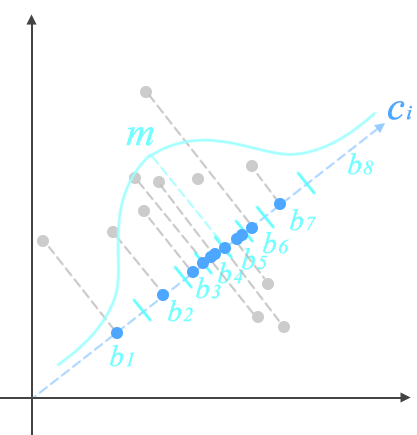
\includegraphics[width=2.5in]{fig_NN/pca_proj.png}
\label{fig:pca-proj}}
\qquad
\subfigure[Dot product distributions]{
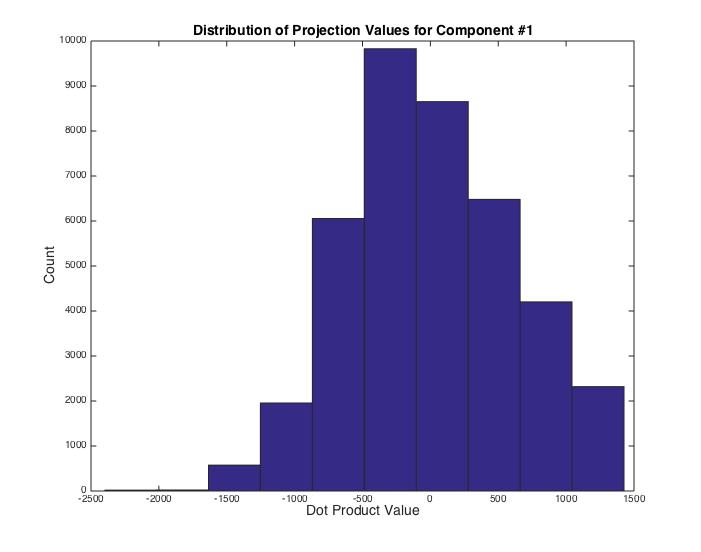
\includegraphics[width=1.0in]{fig_NN/hist_pp1.jpg}
%\vspace{2ex}
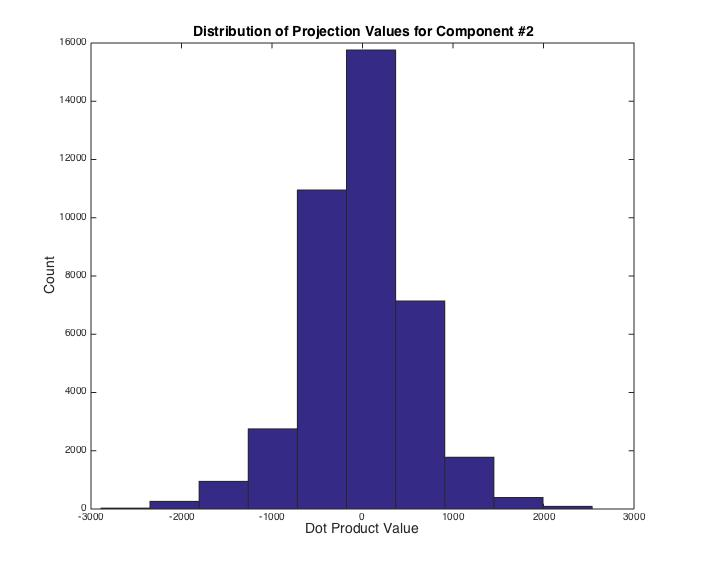
\includegraphics[width=1.0in]{fig_NN/hist_pp2.jpg}
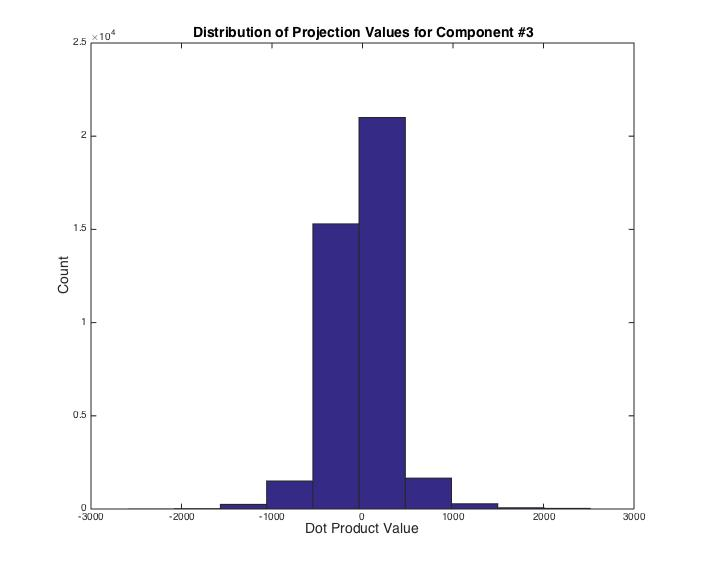
\includegraphics[width=1.0in]{fig_NN/hist_pp3.jpg}
\label{fig:pca-distr}
}
\caption{PCA-based hashing uses directions of maximal
variance in patches as projection vectors, and
adapt the bin size for each projection vector using data.
In b) we show distributions of patch vector projections
on the 3 principal components (magnitude of dot product).}
\label{fig:pca}
\end{figure}

To ensure that patches are well-distributed
among the bins, avoiding database lookup of many potential
neighbors, we propose a \emph{PCA-based hashing scheme}.
Under this scheme, we run Principal Component Analysis (PCA)
to compute directions of largest variance for typical image patches
and use the 10 first principal components as the projection
directions (see fig.~\ref{fig:pca}). This ensures that
the projections of typical patches are as far apart as possible.
To further optimize the binning, we project
a set of patches (grey dots in fig.~\ref{fig:pca}) onto each
principal component $\mathbf{v}_i$ (blue dots in fig.~\ref{fig:pca}), and
approximate the distribution of the dot product
values by a Gaussian $\mathcal{N}_i(\mu_i, \sigma_i)$
(orange curve in fig.~\ref{fig:pca}).
In order to bin a dot product value into one of 8 bins (3 bits/bin),
we adapt the bin size to $\mu_i$ and $\sigma_i$.

\begin{figure}[ht!]
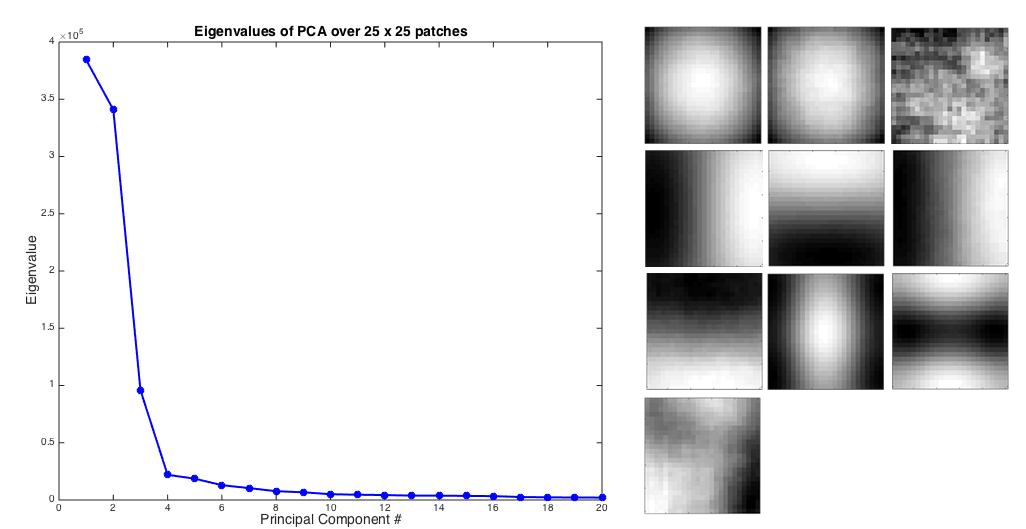
\includegraphics[width=3.0in]{fig_NN/principal_comps.png}
\caption{Eigenvalues of the PCA on 80K patches and visualization
of the L-channel (lightness) of the first 10 components.}
\label{fig:lambdas}
\end{figure}

In our experimental setup we uniformly sampled patches from two distinct
sets of 1000 images from the SUN~\cite{SUN} database
(and distinct from the set of images we inserted into the database),
and used the patches to:
\begin{itemize}
\item compute PCA vectors in Luv color scheme on the \texttt{train{\allowbreak} set}
of 80,000 25x25 patches (see fig.~\ref{fig:lambdas})
\item compute distribution of typical projections on 10
first principal components using the \texttt{dev{\allowbreak} set} of
40,000 25x25 patches (see fig.~\ref{fig:pca-distr}).
\end{itemize}
We found that this choice of a hashing function has \emph{a
significant positive effect on performance} (see sec.~\ref{sec:performance}).

\begin{figure}[ht!]
\subfigure[Pitfalls of standard deviation]{
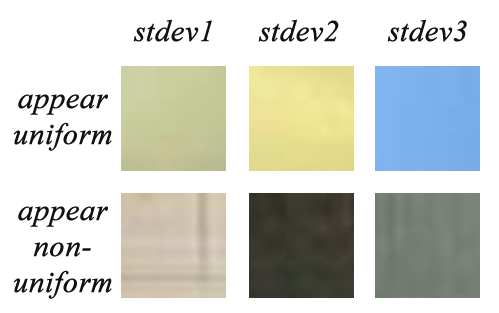
\includegraphics[width=2.5in]{fig_NN/std_uni.png}
\label{fig:color-stdev}}
\subfigure[Uniformity classification with p-norm]{
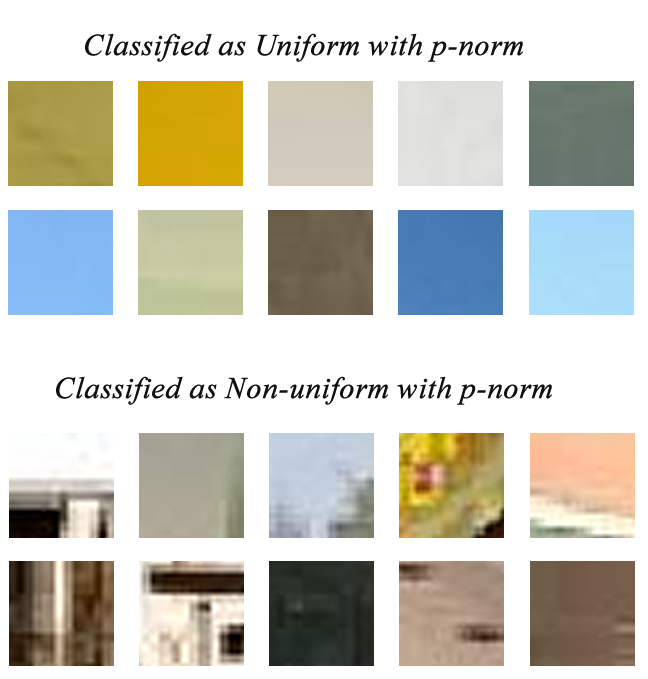
\includegraphics[width=3.0in]{fig_NN/uni_class.png}
\label{fig:color-pnorm}}
\caption{Standard deviation in a) is not very sensitive
to outliers, as patches with nearly identical
values of $stdev1$, $stdev2$ and $stdev3$ may appear
either uniform or non-uniform, as shown in the table.
In b), our classification of patches using
p-norm anecdotally shows more reliable results.}
\end{figure}

\subsection{Hashing Uniform Patches}\label{ssec:uni-nn}

The difficulty of Near Neighbor search for images arises from
their high dimensionality. However, natural images contain many uniform
or nearly uniform patches, which can be easily indexed using
their quantized color. We experimented with using a different
hashing scheme for patches that are nearly uniform, quantizing
them into fewer than 1000 bins by the mean color.

To determine if patch $P$ is uniformly colored, we first
looked at the standard deviation $u_2$ of the patch in all channels, which is
just the L2-norm of $P-\mu(P)$, where $\mu{P}$ is a patch
with every pixel set to the mean of $P$.
However, we found that the L2-norm is insensitive to outliers
(which are very apparent in color patches),
and patches with similar $u_2$ values could appear both uniform
and nonuniform (see fig.~\ref{fig:color-stdev}).

Instead, we decided to classify uniformity using $u_4$, an L4-norm
of $P-\mu(P)$, split into channels. Higher-order forms tend
to collapse all values $< 1.0$ to zero, and expand all values $> 1.0$
to infinity. Hence, we normalize the elements of $P-\mu(P)$ by
our channel threshold $T$ to ensure this property. The best
approach would be to pick uniform thresholds on $u_4$ using
a training set, but in the interest of time we hand-picked
a threshold of $0.1$ for all the channels. See fig.~\ref{fig:color-pnorm}
for results using this classification on a random set of patches.

We evaluate the performance of PCA-based hashing compared to
our hybrid PCA+uniform patch hashing in Sec.~\ref{sec:performance}.
